\documentclass{article}\usepackage[]{graphicx}\usepackage[]{color}
%% maxwidth is the original width if it is less than linewidth
%% otherwise use linewidth (to make sure the graphics do not exceed the margin)
\makeatletter
\def\maxwidth{ %
  \ifdim\Gin@nat@width>\linewidth
    \linewidth
  \else
    \Gin@nat@width
  \fi
}
\makeatother

\definecolor{fgcolor}{rgb}{0.345, 0.345, 0.345}
\newcommand{\hlnum}[1]{\textcolor[rgb]{0.686,0.059,0.569}{#1}}%
\newcommand{\hlstr}[1]{\textcolor[rgb]{0.192,0.494,0.8}{#1}}%
\newcommand{\hlcom}[1]{\textcolor[rgb]{0.678,0.584,0.686}{\textit{#1}}}%
\newcommand{\hlopt}[1]{\textcolor[rgb]{0,0,0}{#1}}%
\newcommand{\hlstd}[1]{\textcolor[rgb]{0.345,0.345,0.345}{#1}}%
\newcommand{\hlkwa}[1]{\textcolor[rgb]{0.161,0.373,0.58}{\textbf{#1}}}%
\newcommand{\hlkwb}[1]{\textcolor[rgb]{0.69,0.353,0.396}{#1}}%
\newcommand{\hlkwc}[1]{\textcolor[rgb]{0.333,0.667,0.333}{#1}}%
\newcommand{\hlkwd}[1]{\textcolor[rgb]{0.737,0.353,0.396}{\textbf{#1}}}%
\let\hlipl\hlkwb

\usepackage{framed}
\makeatletter
\newenvironment{kframe}{%
 \def\at@end@of@kframe{}%
 \ifinner\ifhmode%
  \def\at@end@of@kframe{\end{minipage}}%
  \begin{minipage}{\columnwidth}%
 \fi\fi%
 \def\FrameCommand##1{\hskip\@totalleftmargin \hskip-\fboxsep
 \colorbox{shadecolor}{##1}\hskip-\fboxsep
     % There is no \\@totalrightmargin, so:
     \hskip-\linewidth \hskip-\@totalleftmargin \hskip\columnwidth}%
 \MakeFramed {\advance\hsize-\width
   \@totalleftmargin\z@ \linewidth\hsize
   \@setminipage}}%
 {\par\unskip\endMakeFramed%
 \at@end@of@kframe}
\makeatother

\definecolor{shadecolor}{rgb}{.97, .97, .97}
\definecolor{messagecolor}{rgb}{0, 0, 0}
\definecolor{warningcolor}{rgb}{1, 0, 1}
\definecolor{errorcolor}{rgb}{1, 0, 0}
\newenvironment{knitrout}{}{} % an empty environment to be redefined in TeX

\usepackage{alltt}
\usepackage{Sweave}
\usepackage{float}
\usepackage{graphicx}
\usepackage{tabularx}
\usepackage{siunitx}
\usepackage{mdframed}
\usepackage{natbib}
\bibliographystyle{..//refs/styles/besjournals.bst}
\usepackage[small]{caption}
\setkeys{Gin}{width=0.8\textwidth}
\setlength{\captionmargin}{30pt}
\setlength{\abovecaptionskip}{0pt}
\setlength{\belowcaptionskip}{10pt}
\topmargin -1.5cm        
\oddsidemargin -0.04cm   
\evensidemargin -0.04cm
\textwidth 16.59cm
\textheight 21.94cm 
&\pagestyle{empty} %comment if want page numbers
\parskip 0pt
\renewcommand{\baselinestretch}{1.5}
\parindent 10pt

\newmdenv[
  topline=true,
  bottomline=true,
  skipabove=\topsep,
  skipbelow=\topsep
]{siderules}
\usepackage{lineno}
%\linenumbers
\IfFileExists{upquote.sty}{\usepackage{upquote}}{}
\begin{document}
Concept paper outline:
Green is the color of spring (cite Shwartz nature 1998 Green-wave Phenology), but any keen observer walking the Eastern deciduous forests early in the season would readily notice that it is often the subtle reds and yellows of emerging tree flowers that are the first harbingers of the season. Why do some tree species seasonally flower before leafing out? This trait, known as hysteranthy, is a feature common to deciduous forests that has long been noted by botanists (cite old papers from 1900s), but there has been little empirical investigation into the origins or significance of this phenological pattern. In this paper we aim to:
\begin{itemize}
\item Present and evaluate the current hypotheses relating to the origins and significance of hysteranthy 
\item Develop an empirical framework for identifying hysteranthous species
\item Characterize the prevalence of hysteranthy in Eastern woody species. Identify other plant traits associated with hysteranthy
\item  Discuss the role of hysteranthy for forest demography in a changing climate.
\end{itemize}

\section*{Hysteranthous hypotheses}
\subsection {functional hysteranthy}
\begin{itemize}
\item Wind pollination hypothesis. Evidence: Modeling (cite Whitehead, Niklas), Pollen entrapment by leaves (cite: Lake study).
\item Insect visibility hypothesis. (Cite Janzen). Hysteranthy is also prevalent in the dry deciduous tropics. As far as we know, there is no empirical study testing this.
\item Efficiency investment trade off. Hysteranthous flowers require less investment in attraction. (cite Arboretum Dogwood study)
\item Early flowering. There are good reasons to flower early (cite Bolmgren). Hysteranthous patterns are incidentally created because flowers are "less consequential" compared to leaves over the lifetime of a tree so they can adopt a riskier strategy vis a vis phenologizing in the frosty time of year when compared to their leaves. Both Jessica Savage and Peter Del Tredici mentioned this, but I can't find it anywhere in the literature.
\end {itemize}
\subsection {physiological hysteranthy}
\begin {itemize}
\item genetic architecture require flowering to go first.
\item water constraint. Big flowered species can't get enough water to flowers and leaves at the same time. (Jess Savage told me this but I don't this she's published anything on it yet)
\end{itemize}
With this hypothesizes in mind, we will now discuss some of the challenges for classifying species as hysteranthous.

\section*{Challenges for identifying hysteranthous species}
\subsection*{Hysteranthy literature}
\begin{itemize}
\item Hysteranthy has been described in the literature for over a century but the terms use have varied and may produce unneccisary confusion. Hysteranthy and proteranthy are synonyms that should be antonyms. Though there may be subtle differences (cite paper from Kanchi). Precocious flowering is a synonym but it also means early ontogenetic flowering which makes literature searches difficult. Many sources that discuss this floral-foliate pattern are descriptive with no terminology, which is not conducive for literature searches.
\item We propose using the term hysteranthy. It cannot be confused with a different phenomenon (precocious) and is more general than proteranthy so as to include things like Hamamelis or desert geophytes (cite Dafni and all those other israeli authors who research geophytes) which flower after leaf drop in the fall. We use synanthous to describe flowers that open as leaves are expanding, and seranthous to describe flowers that open after leaves are fully grown. Note: Should/can we define a new term for these floral-foliate patterns in general? (some ideas: folianthy, foliflos-series or just use floral-foliate sequence)
\end{itemize}
\subsection*{Hysteranthy data}
\begin{itemize}
\item Bummer-flowering and leafing phenology are rarely observed together in empirical data sets (cite Lizzie and Ailene). The best sources we have to characterize hysteranthous species are verbal descriptions from guide books and species monographs.  These kinds verbal descriptors, "flowering begins before leaves develop in spring" or "flowers before or with leaves", or incompatible with our current observations standards like bbch scale (cite Finn et al 2007). Does flowering before leaves mean "flower budburst before leaf budburst" (bbch 55 before 09? Does it mean one flower open before one leafout observed (bbch 60 before 15). Does it mean peak flowering before full canopy closure? (bbch 65 before 19)? These criteria would create very different categorizations. For example, using phenological observations from Harvard Forest (cite O'Keefe) we see that if we use flower budburst before leaf budburst, only two species in the community are hysteranthous, while if we use flower open vs. leaves 75percent filled, most of the species are (see figure 1). We do not know what criteria authors of verbal descriptions were using, but they are clearly imprecise, which may explain differences between sources. But differences between sources could as be a product of population or seasonal variation in the degree of hysteranthy which could be significant.  For example, compare seasonal variation of Harvard Forest and Arnold arboretum (treespotters) for Sugar maple or other highly observed tree spotter trees in a figure).
\end {itemize}

\section*{Traits associated with hysteranthy}
\begin{itemize}
\item See data paper draft. Maybe since its a concept paper I can just use MTSV since its a better dataset?
\item Also, demonstrate that how we define hysteranthy matters (the problem we encountered above) to our hypothesis testing. Demonstrate how the effect sizes change when we code hysteranthous as before only before & before/with, before &before/with & with. (This code is done, just would need to be output to the figure)
\end{itemize}

\section*{Towards an empirical definition of Hysteranthy}
Most of the the hypothesizes are functional and related to pollination (1-3 definitely and also kind of 4) so we feel it makes more sense to use a functional definition of hysteranthy. What does that mean? We must have open flowers. We imagine tiny developing leaf primordia won't significantly interfere with wind or insect attraction but as the canopy closes this effect increases. This should definitely be tested. In the meantime, We suggest (60 or 65) should come before (15 or 17) to be considered hysteranthous. This framework will allow for a more detailed characterization of hysteranthous species, help us understand the reaction norms in the patterns based on varying climate conditions.

\section*{Hysteranthy in a changing climate space}
It has been shown that interactions between temperature and day length are cue of both floral and foliar phenology in trees (cite lots of people), and that seasonal temperatures are projected to change dramatically as a result of human industrial activity (cite any reasonable cliamte science). We have already seen shifts in phenology. (cite a lot of people). Will hysteranthy be affected? If foliar and floral phenologies are differential sensitive to changing environmental cues we could see alterations to species floral-foliate sequences in a era of global climate change. If hysteranthy is an adaptive reproductive trait as the hypothesizes suggest, alterations to hysteranthous window might have negative demographic consequences for hysteranthous species. (side bar: is there any data set we could look at to lightly connect masting to hysteranthy?). For example, if the mean leaf free flowering time has been 2 week and leafout accelerates faster than flowering with global warming and the window of leaf free flowering becomes 1 week, plants might experience pollen or dispersal limitation, increased competition for pollinators etc which could ultimate reduce their fitness. (Here, rather than a hypothetical example I could also show the result of Dan Flynn's data for the 3 shrubs, but I am wary of this since I am currently basically reproducing this study.)
We must aim our scientific inquiry to better understand: 
\begin{itemize}
\item The variability of hysteranthy on temporal and spatial scales.
\item The degree of hysteranthy's contribution to pollen limitation,pollen dispersal limits, and seed set.
\item The degree to which flowering and leafing are constrained by each other or independent of each other under changing environmental conditions.
\end{itemize}

\section*{Figures}
\begin{itemize}
\item Harvard forest fuctional vs. physiological hysteranthy plots (already made)
\item Tree spotter hysteranthy interanual variation (Cat made something similar) compared to Harvard forest interanual variation of the same species in the same year.
\item effect size plots for MTSV model.(1 made). Could make 2 more to compare result for other kinds of hysteranthy (ie physiological)
\begin{figure}
    \centering
    \begin{subfigure}
        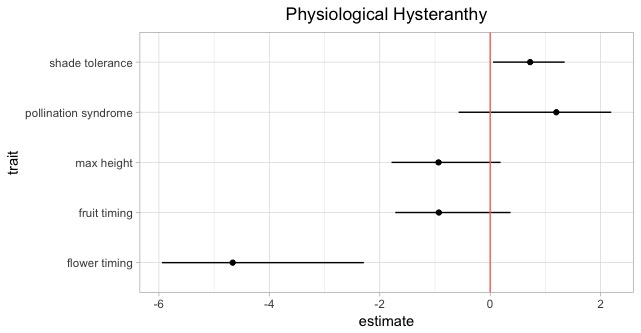
\includegraphics[width=0.8\textwidth]{phys_effect.jpeg}
        \caption{some effect sizes}}
        \label{fig:phys_effect.jpeg}
    \end{subfigure}\begin{subfigure}
        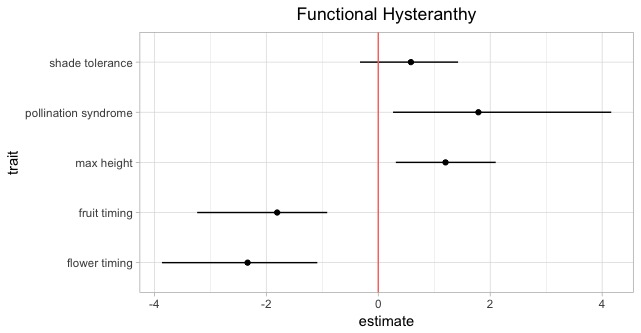
\includegraphics[width=0.8\textwidth]{fuct_effect.jpeg}
        \caption{others}
        \label{fig:fuct_effect.jpeg}
    \end{subfigure}
\end{figure}


\item either conceptual figure of loss of hysteranthy or figure from Dan F's shrubs (alreadt made for CSEE)
\end{itemize}





\end{document}
